%Pengurangan Bilangan Biner dan Heksadesimal
%Kelas: D4 TI 1B
%Alit Fajar Kurniawan(1174057)
%Berlian Nugraha Indra Maha Putra(1174058)
%Ichsan Hizman Hardy(1174034)
%Iqbal Hambali(1174060)
%Kevin Natanael Nainggolan(1174059)
%Virga Ukhu Ismada Yudha(1174065)
%Yusri Rizal(1154072)

\section{pengertian hexadecimal}
	Hexadecimal adalah sebuah sistem bilangan yang menggunakan sebuah simbol.Dalam hexadecimal Terdapat beberapa simbol yang bisa digunakan di sistem bilangan ini.Berbeda dengan bilangan decimal.hexadecimal menggunakan angka 0 sampai 1, di bilangan hexadecimal ini tidak menggunakan angka semua melainkan ada beberapa simbol yang menggunakan huruf.jumlah simbol yang yang berasal dari angka 1 sampai 9 berjumlah 16 simbol, ditambah dengan 6 simbol lainnya yang menggunakan huruf dari A sampai F.Hexadecimal bisa digunakan untuk menampilkan nilai alamat memori dan pemrograman komputer.Teknik penjumlahan dan pengurangan pada bilangan hexadecimal hampir sama dengan penjumlahan dan pengurangan pada bilangan biner,octal dan decimal, tetapi jika terjadi carry 1 atau borrow 1, maka angka 1 tersebut bernilai 16. Carry akan terjadi apabila penjumlahan lebih dari 15 misalnya 8+8=10. Sedangkan borrow terjadi apabila angka yang dikurangi lebih kecil dari pengurang, misalnya 45-6=.
	
	Bilangan heksadesimal yang hanya berbasis 16 memiliki nilai yang dapat disimbolkan dengan 0, 1, 2, 3, 4, 5, 6, 7, 8, 9, A, B, C, D, E, F.
Munculnya bilangan heksadesimal pada operasi komputasi karena apabila operasi bilangan biner untuk data yang lumayan besar akan menjadi 
sulit untuk dibaca, sehingga bilangan heksa selalu digunakan pada saat menggambarkan memori dan instruksi. digunakannya bilang heksa sebagai 
pengganti bilangan biner dikarenakan setiap digit bilangan heksadesimal dapat mewakili 4 bit bilangan binerdan 2 digit bilangan heksa dapat 
mewakili 1 byte 

	Pengurangan pada bilangan heksadesimal

melakukan pengurangan secara berurutan dimulai dari digit yang paling kanan, jika bilangan yang dikurangi lebih sedikit atau lebih kecil 
dari bilangan pengurang maka otomatis bilangan pengurang akan melakukan pinjaman 1 ke bilangan sebelummnya. contoh: 
	
	1. FBC(16) - 321(16) = ..........(16)
 Langkah-langkah penyelesaian: 
FBC 
3 2 1 ----- (-)

C - 1 = 12 -1 = 11, hasil pengurangan adalah B 
B - 2 = 11 - 2 = 9,  hasil pengurangan adalah 9
F - 3 = 15 - 3 = 12, hasil pengurangan adalah C 

Jadi hasil pengurangannya adalah  FBC(16) - 321(16) = C9B(16) 

	2. b.	F30(16) – D89(16) =  ..........(16)
Penyelesaian :
1.	0 – 9,karena angka 0 lebih kecil dari 9 maka terjadi borrow 1 yang bernilai 16 yang membuat angka 0 menjadi 16 dari 0+16. Hasil pengurangan 16 – 9 = 7.
2.	2 – 8,karena telah terjadi borrow 1 pada sebelumnya maka angka 3 – 1 = 2. Karena angka 2 lebih kecil dari 8 maka terjadi borrow 1 yang membuat angka 2 menjadi 18 dari 2+16. Hasil pengurangan 18 – 8 = 10 atau .
3.	E – D = 14 – 13 = 1,E berasal dari F yang dikurangi 1 karena telah terjadi borrow pada sebelumnya.
Hasil pengurangan dari F30(16) – D89(16) = 1A7(16).
	
\subsection{operasi pengurangan pada bilangan hexadesimal}
pengurangan mudah diselesaikan jika dikerjakan dengan rapi yaitu memperhatikan lajur-lajur perseratusan, persepuluhan, satuan, puluhan, ratusan, dan sebagainya. untuk menyelesaikan pengurangan bilangan hexadesimal, ikuti langkah-langkah ini: 1)tulis kedua bilangan bersusun ke bawah, sejajarkan sehingga koma hexadesimal membentuk baris lurus, 2) tambahkan nol agar bilangan memiliki panjang yang sama, 3) kemudian kurangkan, jangan lupa mencantumkan koma hexadesimal pada jawabannya.

\begin{figure}[ht]
\centerline{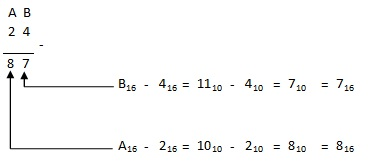
\includegraphics[width=0.1\textwidth]{figures/heksadesimal.jpg}}
\caption{Pengurangan Heksadesimal}
\label{Bilangandesimal}
\end {figure}

\section {Bilangan Biner atau Binary}
Bilangan Binary Pada saat pertama kali komputer atau elektronik digunakan,sistem operasinya telah menggunakan bilangan biner (Binary),yaitu bilangan dengan basis 2 pada system bilangan. Semua perhitungan diolah menggunakan aritmatik biner,yaitu bilangan yang hanya memiliki dua nilai kemungkinan 0 dan 1 yang biasa disebut bit (binary digit). Semua kode program dan data disimpan dalam format biner yang merupakan sebuah kode-kode dari komputer. Pada setiap posisi memiliki bobot nilai yang berbeda,dimana pada posisi paling depan (kiri) memiliki nilai yang paling besar yang biasa disebut MSB (Most Significant Bit) dan pada posisi paling belakang (kanan) memiliki nilai paling kecil yang biasa disebut LSB (Leased Significant Bit).
	
\subsection {Operasi Pengurangan Bilangan Biner}	
	Pengurangan Bilangan Biner
	contoh :
Kondisi yang muncul pada pengurangan bilangan biner (0-0,0-1,1-0,1-1) dimana :
0 – 0 = 0
0 – 1 = 1 borrow 1 (jika masih ada angka di sebelah kiri)
1 – 0 = 1
1 – 1 = 0
penjelasannya: maksudnya meminjamkan satu digit angka dari kolom sebelah yang memiliki nilai lebih besar dari hasil pengurangan mencukupi.
Contoh pada bilangan biner :
1100010 – 110111 = 0101011 
Contoh pada bilangan decimal :
37 – 32 = 5 (borrow 0)
23 – 17 = 6 (3 borrow 1 dari angka 2)
Pada perhitungan pertama tidak ada proses meminjam (borrow) angka yang lebih besar karena hasil pengurangan di digit belakang sudah mencukupi untuk dikurangkan dengan bilangan pengurangnya ,sementara pada perhitungan ke-2 ada proses peminjaman karena 3 tidak mencukupi dikurangkan dengan 7.

\begin{figure}[ht]
\centerline{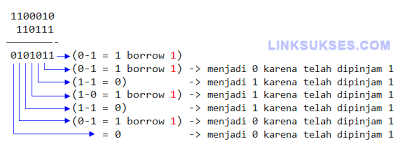
\includegraphics[width=0.1\textwidth]{figures/PenguranganBiner.jpg}}
\caption{Pengurangan Bilangan Biner}
\label{BilanganBiner}
\end {figure}

\section {cara Mengkonversikan Bilangan}
 CARA MENKONVERSIKAN BILANGAN BINARY MENJADI BILANGAN HEXADESIMAL
 
 konversi yang berawal dari bilangan binary menjadi bilangan hexadesimal sama saja caranya dengan ketika akan mengkonversikan bilangan binary kebilangan oktal. pada awalnya melakukan pembagian pada bilangan binary supaya menjadi beberapa kelompok, yang masing-masing kelompokya mempunyai maksimal 4 digit, dimulai dari bilangan binary paling kanan.
contoh:
 
apa bila jumlah angkanya hanya 2 digit seperti 11 maka pangkatnya hanya 0 dan 1. begitu juga dengan angka 1010 yang ada 4 digit, berarti pangkatnya 0, 1, 2, 3 . 
misal: angkanya 11 maka menjadi
		1*2 pangkat 0
		1*2 pangkat 1
		begitu juga dengan yang lainnya.


MENGKONVERSIKAN BILANGAN HEXADESIMAL KE BILANGAN BINARY

Untuk mengkonversikannya kita hanya perlu mengkonversikan masing-masing dari perdigit nya, cara konversinya sama dengan mengkonversikan bilangan desimal ke bilangan binary.
contoh: 
	5/2=2, sisanya 1
	2/2=1, sisanya 0
	1/2=0, sisanya 1
	
karena kita memerlukan empat digit, maka kita memerlukan bilangan binary 0101 sebagai konversi dari desimal 5.

Cara untuk mengkonversi bilangan biner ke oktal dapat dilakukan dengan mengkonversi tiga buah digit biner. Dapat dilihat pada gambar \ref{konversioktal} untuk dapat merubah bilangan biner ke bilangan oktal, kita harus perhatikan bahwa pada setiap bilangan oktal mewakili 3 bit dari bilangan biner. Jadi, jika kita temukan bilangan biner 111110 dikonversikan ke bilangan oktal, langkah awak yang harus dilakukan adalah membagi-bagi bilangan biner tersebut, pada setiap bagian 3 bit, dapat dimulai dari sebelah Kanan ke Kiri, hingga menjadi seperti ini : 111 110 yang jika di koversikan ke dalam oktal maka hasil yang di dapat adalah 76 dalam bilangan oktal.

\subsubsection{Konversi Sistem Bilangan Biner ke Desimal}
Bilangan Biner dapat dikonversikan ke bentuk desimal dengan cara mengalikan satu-satu bilangan atau dengan dua basis biner pangkat 0 dan pangkat 1. Mengalikan bit dalam bilangan dengan position valuenya.Bilangan bineri 11001 dapat dikonversikan ke dalam bentuk desimal senilai : \\

\begin{equation}
11001_{2} = (1x20)+(0x21)+(0x22)+(1x2)+(1x22) \\
= 1+0+0+8+16 
= 25
\end{equation}

\subsubsection{Konversi Bilangan Biner ke Bilangan Hexadesimal}
Konversi bilangan biner ke bilangan hexadesimal hampir mirip seperti Konversi pada bilangan oktal. Hanya saja pada bilangan hexadesimal memakai 4 digit angka yang diambil dari bilangan biner.Selain itu untuk nilai yang lebih besar dari 9 dapat diganti dengan huruf Heksadesimal seperti A,B,C,D sampai H. 
\subsection{Bilangan Oktal}
Bilangan oktal adalah sistem bilangan yang berbasis 8 dan mempunyai delapan simbol bilangan yang berbeda : 0,1,2,...,7.
Teknik pembagian yang berurutan dapat menggunakan untuk mengubah bilangan desimal menjadi bilangan oktal. Bilangan desimal yang akan diubah secara berturut-turut dibagi dengan 8 dan sisa pembagian harus selalu dicatat. 
\subsubsection{Konversi Bilangan Oktal ke Bilangan Biner}
Cara ini merupakan kebalikan cara konversi biner ke oktal. Setiap digit oktal akan langsung dikonversi ke biner lalu hasilnya digabungkan.
\\contoh:
\\548 = …….2 ?
\\
\begin{enumerate}
\item Pertama-tama hitung 58 = 1012 (Lihat cara konversi dari desimal ke biner)
\item Lalu hitung 48 = 1002
\item Sehingga didapat 548 = 1011002
\item Anda juga dapat menggunakan rumus di ms excel OCT2BIN() yang akan menkonversi bilangan oktal ke biner
\end{enumerate}

\subsubsection{Konversi Oktal ke Desimal}
Cara untuk mengkorvesikan bilangan oktal ke heksadesimal yaitu dengan mengkonveksikan bilangan oktal tersebut ke biner terlebih dahulu kemudian bilangan tersebut di konveksikan ke heksadesimal. Untuk lebih jelasnya, perhatikan contoh konveksi bilangan oktal ke heksadesimal sebagai berikut:
\\ Contoh konversi oktal ke heksadesimal:
\begin{equation}
\\357_{8}=......_{16} 357 \end{equation}oktal sama dengan berapa bilangan heksadesimal?
Adapun cara pengerjaannya sebagai berikut adalah:
\begin{enumerate}
\item Kita pisahkan 357 menjadi 3, 5, dan 7 kemudian konversikan ke biner 
\item 3 = 011 5=101 7=111
\item Setelah dapat biner nya yaitu 011101111 kemudian konversi biner tersebut ke heksadesimal. 
\item 011101111 -------- 1111 = 15 = F 1110 = 14 = E 0 = 0
\item Maka di dapat bahwa 357 oktal sama dengan EF hexadesimal 
\end{enumerate}

\section{Fungsi dari Konversi Bilangan}
Membuat sebuah program tidak hanya membutuhkan bahasa pemrograman. Pada bagian komputernya juga memerlukan sebuah bahasa yang dimengerti oleh komputer tersebut. yaitu bilangan biner. jadi salah satu Fungsi dari konversi bilangan ini salah satunya adalah untuk membuat sebuah program. Selain memakai sebuah sistem bilangan desimal, pembuatan sebuah program itu terkadang juga menggunakan bilangan biner, oktal, dan hexadesimal.
Fungsi lain dari Konversi bilangan ini salah satunya adalah untuk membaca sebuah perintah yang dimana perintah tersebut masih menggunakan perintah yang hanya bisa dibaca oleh komputer yaitu Biner. tetapi dengan adanya Konversi Bilangan, Sebuah angka tersebut bisa dijadikan sebagai suatu line perintah bahkan sebuah kata yang nantinya dapat dimunculkan oleh komputer kepada pengguna. Pembuatan aplikasi sendiri membutuhkan sebuah Konversi Bilangan yang nantinya akan menggerakan sebuah modul - modul dalam sebuah perangkat yang dipakai dalam aplikasi tersebut. 
Konversi Sendiri dilakukan dalam sebuah Processor atau ALU yang mereka hanya dapat membaca kode biner yang nantinya saat setelah diproses akan dimasukan ke memori yang nanti akan dikonversi ditampilkan ke layar dengan berbentuk yang sesuai dengan yang dibutuhkan \cite{noersasongko1996mengrnal}
\\Membuat sebuah program tidak hanya membutuhkan bahasa pemrograman. Pada bagian komputernya juga memerlukan sebuah bahasa yang dimengerti oleh komputer tersebut. yaitu bilangan biner. jadi salah satu Fungsi dari konversi bilangan ini salah satunya adalah untuk membuat sebuah program. 
\\Fungsi lain dari Konversi bilangan ini salah satunya adalah untuk membaca sebuah perintah yang dimana perintah tersebut masih menggunakan perintah yang hanya bisa dibaca oleh komputer yaitu Biner. tetapi dengan adanya Konversi Bilangan, Sebuah angka tersebut bisa dijadikan sebagai suatu line perintah bahkan sebuah kata yang nantinya dapat dimunculkan oleh komputer kepada pengguna. Pembuatan aplikasi sendiri membutuhkan sebuah Konversi Bilangan yang nantinya akan menggerakan sebuah modul - modul dalam sebuah perangkat yang dipakai dalam aplikasi tersebut. 

\section{Penerapan Konversi Bilangan}
Konversi Bilangan diterapkan khususnya pada bidang Teknologi. Selain sebagai instruksi, Konversi sendiri dapat dikenal sebagai pengenal dalam situasi tertentu. seperti untuk mengenal warna dan sebagainya. Beberapa contoh dari penerapan tersebut adalah sebagai berikut : 
\begin{itemize}
\item Sebagai kode warna dalam pemrograman \\ Konversi Bilangan sering sekali dipakai untuk mengetahui berapa tingkat warna dan seberapa pekat warna tersebut. Konversi Bilangan pada kasus ini menggunakan Konversi Desimal ke Heksadesimal dimana warna terbagi menjadi Merah, Hijau, Biru. 
\item Sebagai Penampil Angka dalam Kalkulator \\ Dengan adanya Konversi Bilangan, Angka yang dikirimkan ke memori akan diubah kedalam bentuk angka biner yang sebelumnya dikonversi dengan menekan sebuah tombol yang mengirimkan aliran kepada memori untuk mengirimkan angka biner.
\item Untuk menampilkan hasil perhitungan dari ALU \\ Pada ALU, Bilangan yang dipakai adalah bilangan Biner yang sangat kecil memungkinkan untuk dibaca oleh computer atau monitor pada umumnya. Oleh karena itu, Untuk menampilkan hasil dari perhitungan, Dibutuhkan sebuah konversi yang dilakukan setelah proses perhitungan mengeluarkan sebuah hasil yang nanti akan ditampilkan oleh Monitor.
\end{itemize}

\cite {Sriwasito, Putut}
\cite {Hutahaean, Jeperson}
\cite {Gulo, Famalua)}